\clearpage
\onecolumn
\begin{landscape}
	\section{Anhang}
	\subsection{Approximation des Bode-Diagramms}\label{approx_bode}
	\renewcommand{\arraystretch}{1.5}
	\begin{longtable}{|p{5cm}|l|ll|ll|}
		\hline
		\textbf{Pole} & 
		\textbf{UTF} $H(s)$ &
		\multicolumn{2}{c}{\textbf{Amplitude} $|H(s)|$} & 
		\multicolumn{2}{|c|}{\textbf{Phase} $\angle(H(s))$}
		\\ \hline
		Keine, konstanter Faktor &
		$\alpha e^{j \beta}$ &
		\parbox[c][1cm]{1cm}{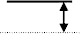
\includegraphics[width=1cm]{Images/bode-approx-konst.png}} &
		\, Konstant: $20 \log \alpha$ &
		\parbox[c][1cm]{1cm}{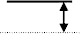
\includegraphics[width=1cm]{Images/bode-approx-konst.png}} &
		Konstant: $\beta$
		\\ \hline
		Pol im Ursprung &
		$\frac{\alpha}{s}$ &
		\parbox[c][1cm]{1cm}{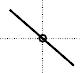
\includegraphics[width=1cm]{Images/bode-approx-ampl-tp-ord1.png}} & 
		\begin{tabular}{l}
			Lineare Steigung: $-20 dB/Dek.$ \\
			$0dB$ bei $\omega = \alpha$
		\end{tabular} &
		\parbox[c][1cm]{1cm}{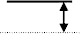
\includegraphics[width=1cm]{Images/bode-approx-konst.png}} & 
		Konstant: $-\frac{\pi}{2}$ 
		\\ \hline
		Nullstelle im Ursprung &
		$\alpha s$ &
		\parbox[c][1cm]{1cm}{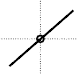
\includegraphics[width=1cm]{Images/bode-approx-ampl-hp-ord1.png}} & 
		\begin{tabular}{l}
			Lineare Steigung: $+20 dB/Dek.$ \\
			$0dB$ bei $\omega = \frac{1}{\alpha}$
		\end{tabular} &
		\parbox[c][1cm]{1cm}{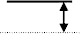
\includegraphics[width=1cm]{Images/bode-approx-konst.png}} &
		Konstant: $+\frac{\pi}{2}$
		\\ \hline	
		Reeller Pol (TP 1.Ord) &
		$\frac{1}{s + \alpha}$ &
		\parbox[c][1cm]{1cm}{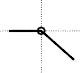
\includegraphics[width=1cm]{Images/bode-approx-ampl-4.png}} &
		\begin{tabular}{ll}
			$\omega < \alpha$: & Konstant $-20 \log \alpha$  \\
			$\omega > \alpha$: & $-20dB/Dek.$
		\end{tabular} &
		\parbox[c][1cm]{1cm}{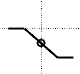
\includegraphics[width=1cm]{Images/bode-approx-phase-4.png}} &
		\begin{tabular}{ll}
			$\omega < \frac{\alpha}{10} $:	& Konstant $0$ \\
			$\omega > 10 \alpha$:		& Konstant $-\frac{\pi}{2}$
		\end{tabular}
		\\ \hline
		Reeller Pol (TP 1.Ord) &
		$\frac{\alpha}{s + \alpha}$ &
		\parbox[c][1cm]{1cm}{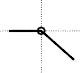
\includegraphics[width=1cm]{Images/bode-approx-ampl-4.png}} &
		\begin{tabular}{ll}
			$\omega < \alpha$: & Konstant $0dB$ \\
			$\omega > \alpha$: & $-20dB/Dek. \qquad (\omega_r = \alpha)$
		\end{tabular} &
		\parbox[c][1cm]{1cm}{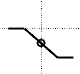
\includegraphics[width=1cm]{Images/bode-approx-phase-4.png}}	& 
		\begin{tabular}{ll}
			$\omega < \frac{\alpha}{10}$: & Konstant $0$ \\
			$\omega > 10 \alpha$: & Konstant $-\frac{\pi}{2}$
		\end{tabular}
		\\ \hline
		Reelle Nullstelle (HP 1.Ord) &
		$s + \alpha$ & 
		\parbox[c][1cm]{1cm}{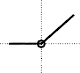
\includegraphics[width=1cm]{Images/bode-approx-ampl-5.png}} &
		\begin{tabular}{ll}
			$\omega < \alpha$: & Konstant $20 \log \alpha$ \\
			$\omega > \alpha$: & $+20dB/Dek.$
		\end{tabular} & 
		\parbox[c][1cm]{1cm}{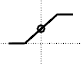
\includegraphics[width=1cm]{Images/bode-approx-phase-5.png}}	&
		\begin{tabular}{ll}
			$\omega < \frac{\alpha}{10}$: & Konstant $0$ \\
			$\omega > 10 \alpha$: & Konstant $+\frac{\pi}{2}$
		\end{tabular}
		\\ \hline	
		Reelle Nullstelle (HP 1.Ord) &
		$\frac{s + \alpha}{\alpha}$ &
		\parbox[c][1cm]{1cm}{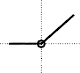
\includegraphics[width=1cm]{Images/bode-approx-ampl-5.png}} &
		\begin{tabular}{ll}
			$\omega < \alpha$: & Konstant $0dB$ \\
			$\omega > \alpha$: & $+20dB/Dek.$
		\end{tabular} &
		\parbox[c][1cm]{1cm}{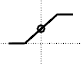
\includegraphics[width=1cm]{Images/bode-approx-phase-5.png}} &
		\begin{tabular}{ll}
			$\omega < \frac{\alpha}{10}$: & Konstant $0$ \\
			$\omega > 10 \alpha$: & Konstant $+\frac{\pi}{2}$
		\end{tabular}
		\\ \hline
		Konjugiert-komplexe Pole \newline
		für $|q_p| > 1/2$ (TP 2.Ord) &
		$\frac{1}{s^2+s\frac{\omega_p}{q_p}+\omega_p^2}$ &
		\parbox[c][1cm]{1cm}{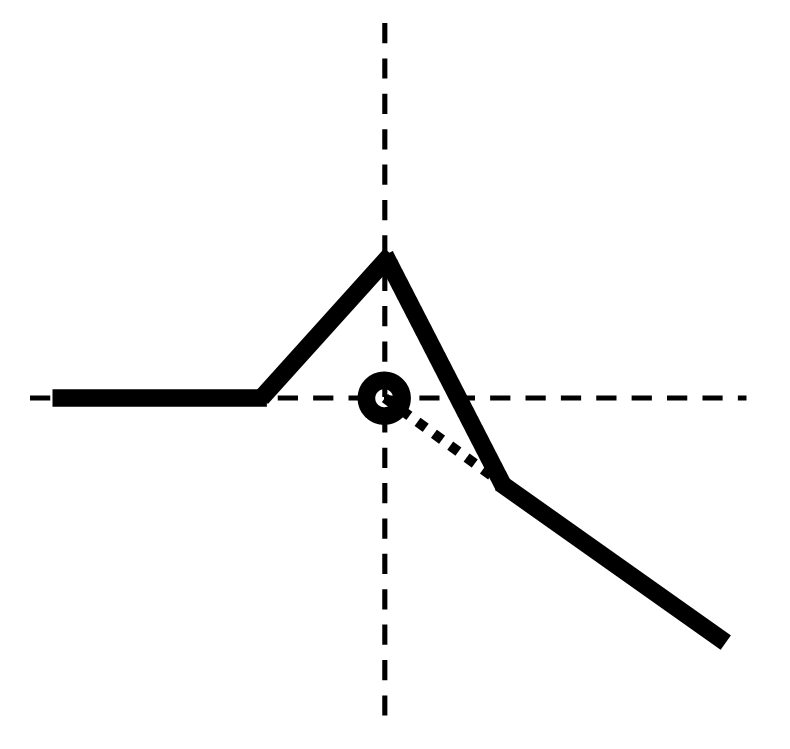
\includegraphics[width=1cm]{Images/bode-approx-ampl-6.png}} &
		\begin{tabular}{ll}
			$\omega < \omega_p$: 	& Konstant $-40 \log \omega_p$ \\
			$\omega > \omega_p$:	& $-40dB/Dek.$ \\
			Überhöhung: 			& $\frac{\omega_p}{2}$ bis $2\omega_p$ \\
			Maximum:				& $-40\log\omega_p + 20 \log q_p$ bei $\omega = \omega_p$			
		\end{tabular} &
		\parbox[c][1cm]{1cm}{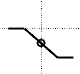
\includegraphics[width=1cm]{Images/bode-approx-phase-6.png}} &
		\begin{tabular}{ll}
			$\omega < \frac{\omega_p}{10^{\frac{1}{2q_p}}}$:	& Konstant $0$ \\
			$\omega > \omega_p 10^{\frac{1}{2q_p}}$:			& Konstant $-\pi$ \\
			$\omega = \omega_p$:								& $-\frac{\pi}{2}$
		\end{tabular}
		\\ \hline
		Konjugiert-komplexe Pole \newline
		für $|q_p| > 1/2$ (TP 2.Ord)&
		$\frac{\omega_p^2}{s^2+s\frac{\omega_p}{q_p}+\omega_p^2}$ & 
		\parbox[c][1cm]{1cm}{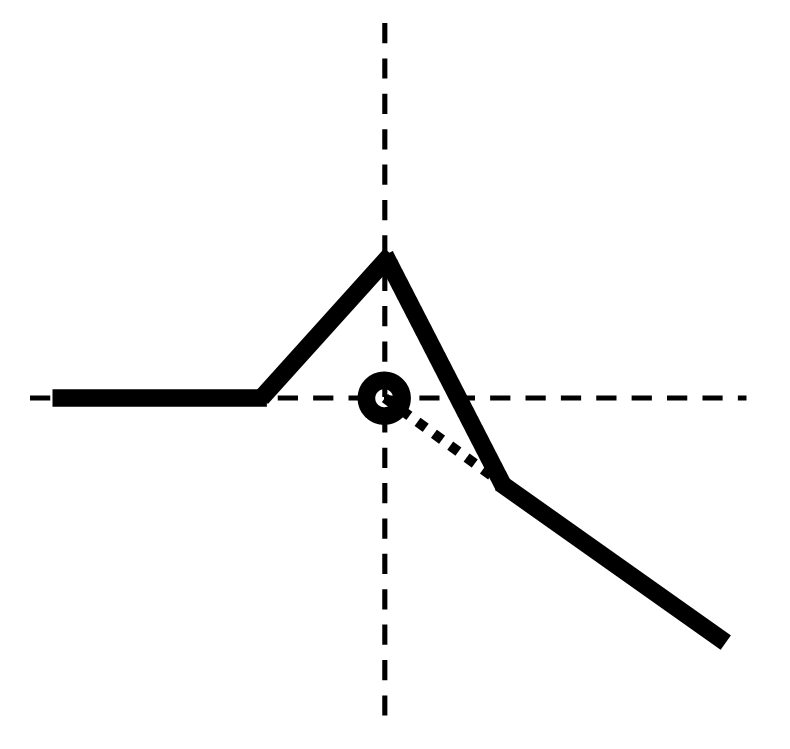
\includegraphics[width=1cm]{Images/bode-approx-ampl-6.png}} &
		\begin{tabular}{ll}
			$\omega < \omega_p$:	& Konstant $0dB$ \\
			$\omega > \omega_p$:	& $-40dB/Dek.$ \\
			Überhöhung:				& $\frac{\omega_p}{2}$ bis $2 \omega_p$ \\
			Maximum:				& $20 \log q_p$ bei $\omega = \omega_p$
		\end{tabular} &
		\parbox[c][1cm]{1cm}{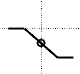
\includegraphics[width=1cm]{Images/bode-approx-phase-6.png}}	& 
		\begin{tabular}{ll}
			$\omega < \frac{\omega_p}{10^{\frac{1}{2q_p}}}$:	& Konstant $0$ \\
			$\omega > \omega_p 10^{\frac{1}{2q_p}}$:			& Konstant $-\pi$ \\
			$\omega = \omega_p$:								& $-\frac{\pi}{2}$
		\end{tabular}
		\\ \hline	
		Konjugiert-komplexe Nullstellen
		für $|q_z| > 1/2$ (HP 2.Ord)&
		$s^2+s\frac{\omega_z}{q_z}+\omega_z^2$ &
		\multicolumn{4}{l|}{
			Analog zu den Konjugiert-komplexen Polen jedoch gespiegelt an der $0dB$- / $0$-Grad-Linie.
  		}
		\\
		&
		$\frac{s^2+s\frac{\omega_z}{q_z}+\omega_z^2}{\omega_z^2}$ &
		\multicolumn{4}{l|}{}
		\\ \hline
		\multicolumn{6}{|p{21cm}|}{
			Serieschaltung von Systemen erfolgt durch \textbf{Superposition} der einzelnen Bode-Diagramme 
			(Multiplikation von UTFs entspricht Addition im	dB-Bereich). $\alpha , \beta \in \mathbf{R}$. 
			Für $\omega_p$ und $q_p$ siehe Kapitel \ref{frequenzgang}
		}
		\\ \hline
	\end{longtable}
	\renewcommand{\arraystretch}{\arraystretchOriginal}
\end{landscape}
\clearpage
\twocolumn

\subsection{PN und Bode von UTF}\label{pn}
\begin{center}
	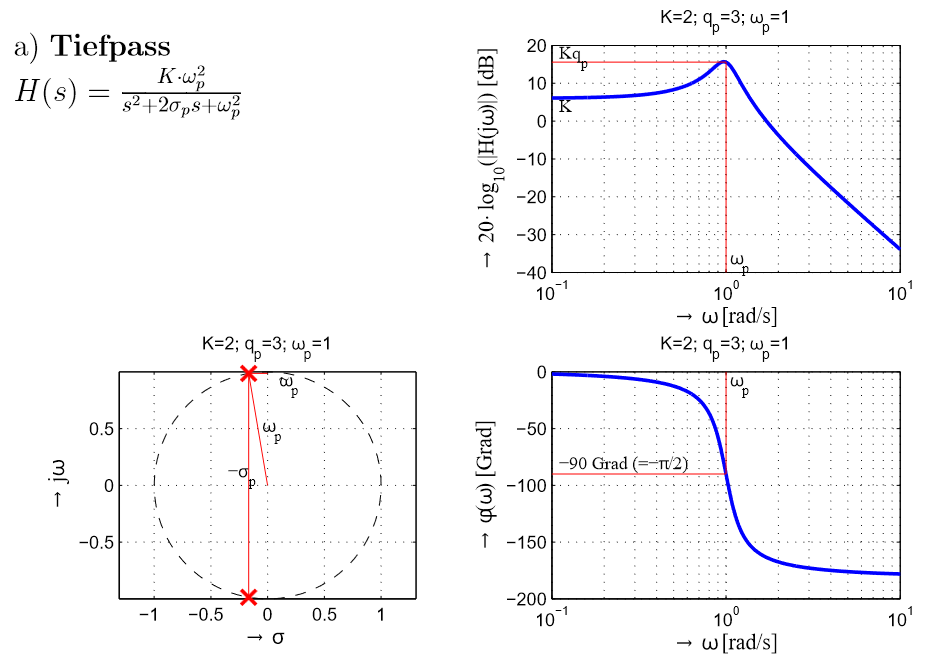
\includegraphics[width=0.8\columnwidth]{Images/tiefpass}\\
	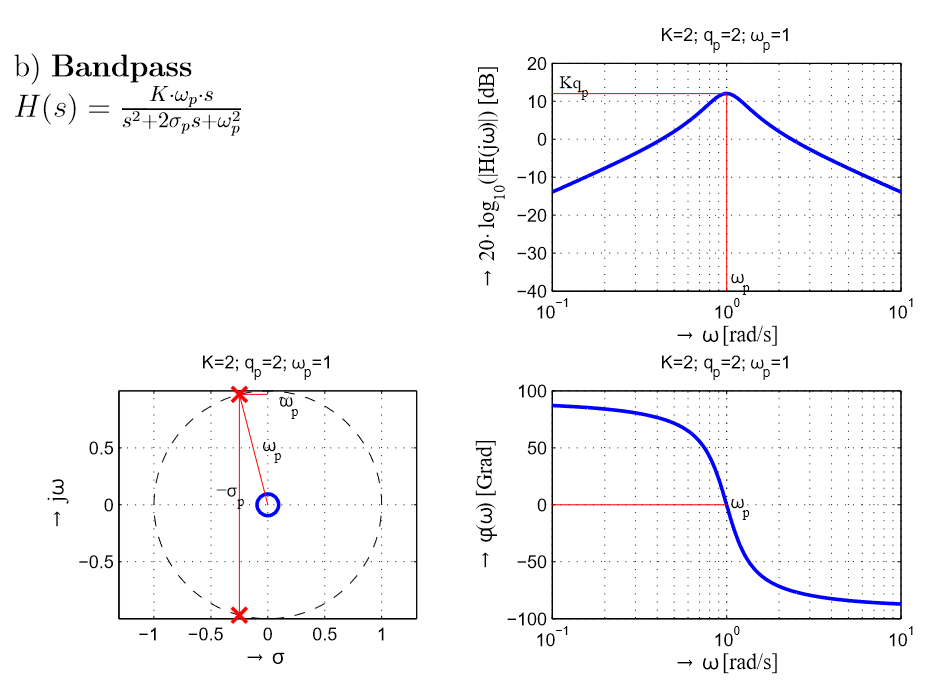
\includegraphics[width=0.8\columnwidth]{Images/bandpass}\\
	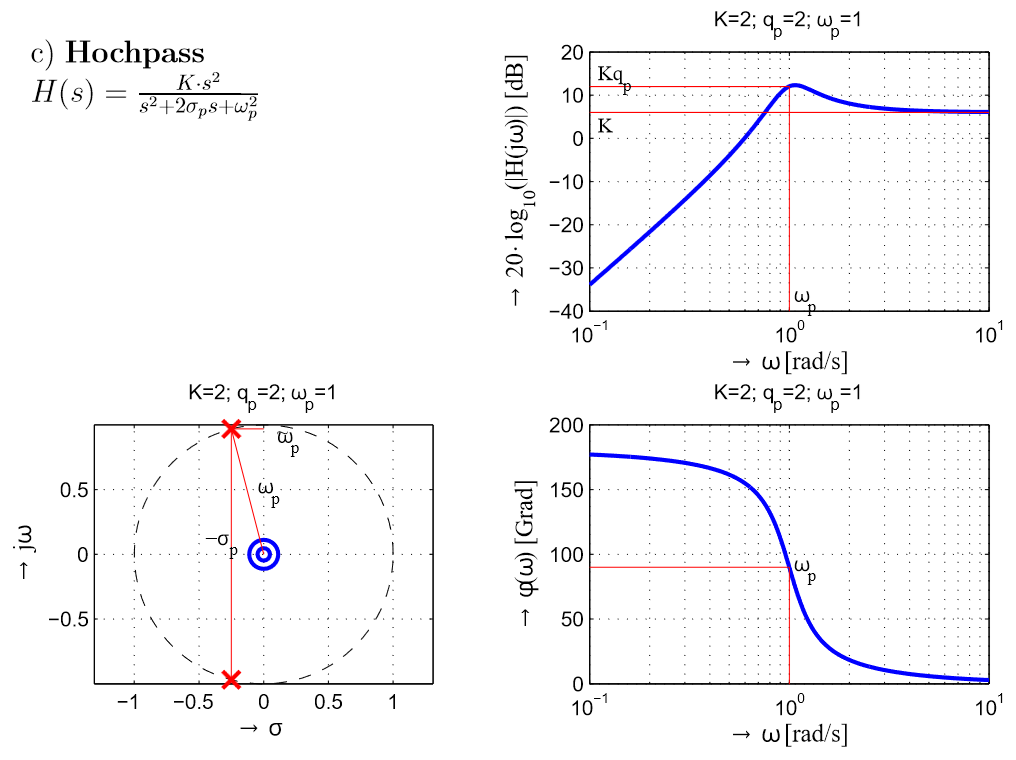
\includegraphics[width=0.8\columnwidth]{Images/hochpass}\\
	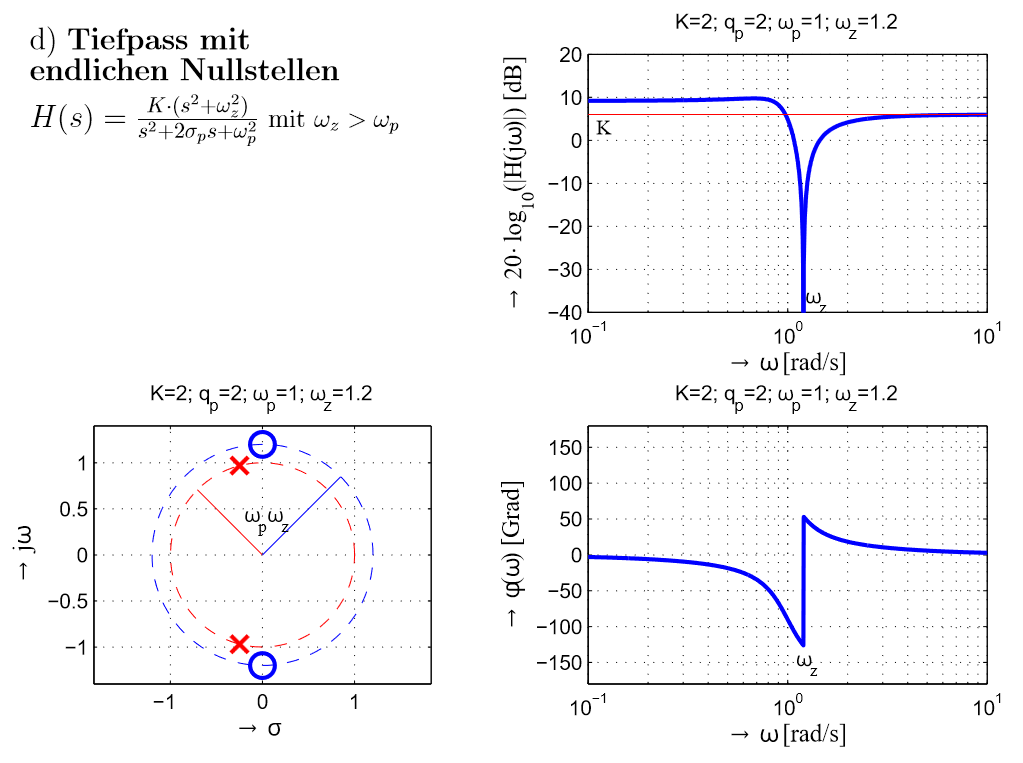
\includegraphics[width=0.8\columnwidth]{Images/tiefpass_en}\\
	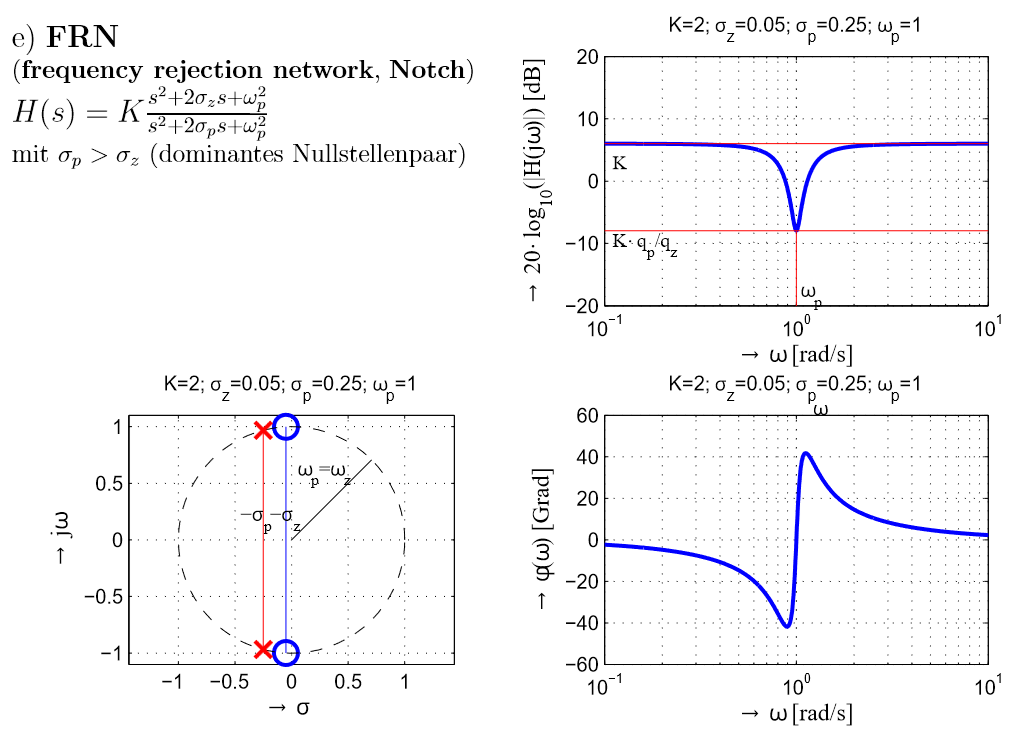
\includegraphics[width=0.8\columnwidth]{Images/frn}\\
	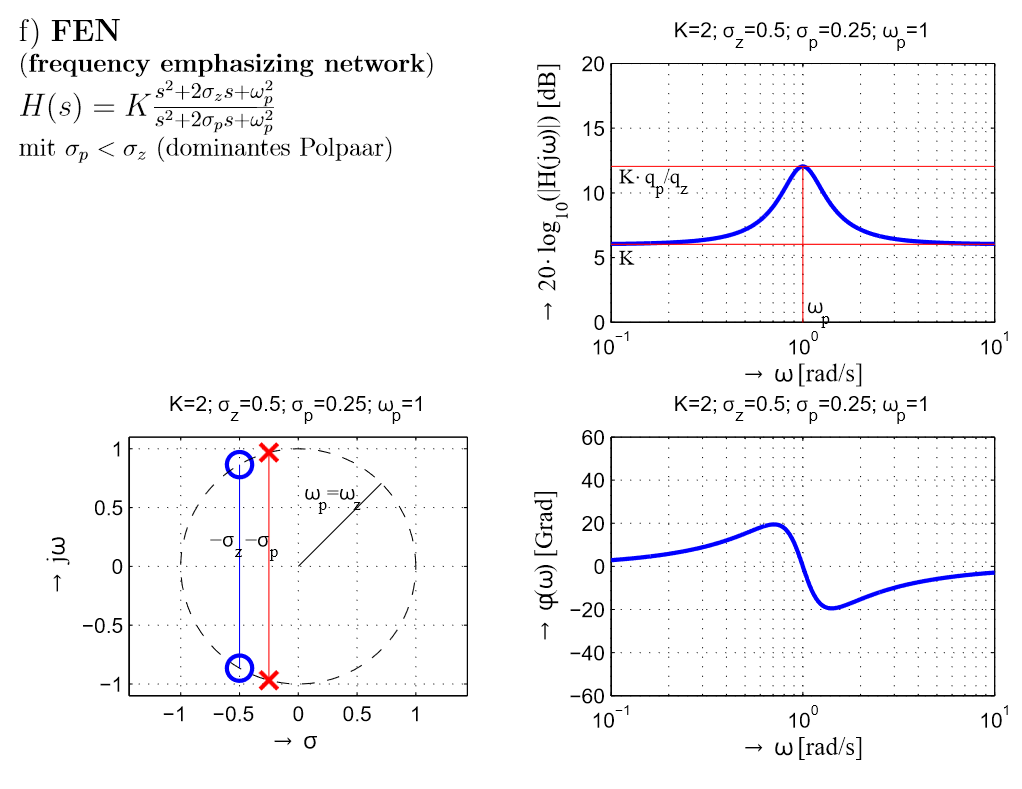
\includegraphics[width=0.8\columnwidth]{Images/fen}\\
\end{center}

\subsection{Filter Übersicht}
\begin{center}
	\rotatebox{90}{
		\bgroup
		\def\arraystretch{2.5}
\begin{tabular}{r|c|c|c|c|c|c}
	& \textbf{Krit. gedämpft}           & \textbf{Butterworth}                     & \textbf{Chebyshev 1}          & \textbf{Chebyshev 2}            & \textbf{Cauer}    & \textbf{6}         \\\hline
	\textbf{Allpolfilter} & Ja                       & Ja                              & Ja                   & Nein                   & Nein     & Ja             \\\hline
	\textbf{Pollage}      & reelle Achse \textless 0 & Halbkreis LHE                   & Ellipse LHE          & LHE                    & LHE      & exentr. Kreis  \\\hline
	\textbf{NS-Lage }     & -                        & -                               & -                    & jw-Achse               & jw-Achse & -              \\\hline
	\textbf{DB}           & streng monoton           & streng monoton (steilstmöglich) & Wellig, konst Rippel & Streng monoton         & wellig   & streng monoton \\\hline
	\textbf{SB}           & Streng monoton           & string monoton                  & Streng monoton       & Weillig, konst. Rippel & wellig   & Streng monoton \\\hline
	\textbf{Phasengang}   & sehr gut                 & mittel                          & schlecht             & schlecht               & wild     & best möglich          
\end{tabular}
	\egroup
}
\end{center}